\section{Where the earlier attempt fails}\label{sec:earlier}

The preprint \cite{BB26} of the two authors claimed the conjecture in full. We record here each point at which it fails, so that the present paper can be read as its replacement and not as a continuation. Numbers refer to that preprint.

\paragraph{The secant cycle (Definition 3, Lemma 4).} For an abelian $2n$-fold $A$ of Weil type the preprint takes $\Sigma=\mathrm{Sec}^{n}(A^{\vee})$, the closure of the union of the $(n-1)$-planes spanned by $n$ points of $A^{\vee}$ in a projective embedding, and the cycle $Z_{\Sigma}=\Sigma\cap A^{\vee}$, asserted to have codimension $n$. Every point of $A^{\vee}$ lies on such a plane, so $A^{\vee}\subseteq\Sigma$ and $Z_{\Sigma}=A^{\vee}$: the intersection is not proper. The sheaf $\mathcal{O}_{\Sigma}|_{A^{\vee}}$ is $\mathcal{O}_{A^{\vee}}$, whose Fourier--Mukai transform is the skyscraper sheaf at the origin shifted by $-2n$, with Chern character the class of a point. So $\ch_{k}=0$ for $1\le k<2n$, contrary to Lemma~4, and Proposition~2 has nothing to identify with a Weil class.

\paragraph{The polarisation (Definition 3).} The polarisation is taken principal, so $\chi(L)=1$ and the embedding is into $\PP^{0}$; the dimension count needs $\chi(L)=2n^{2}+2n$. A principal polarisation is never very ample.

\paragraph{The dimension of the Weil space (Proposition 1).} $\det_{K}H^{1}(A)$ is a two-dimensional $\QQ$-space of Hodge classes \cite{Weil77}, so at a very general point $\Hdg^{n}(A)=\QQ\eta^{n}\oplus W(A)$ has dimension three, not two.

\begin{figure*}[t]
\centering
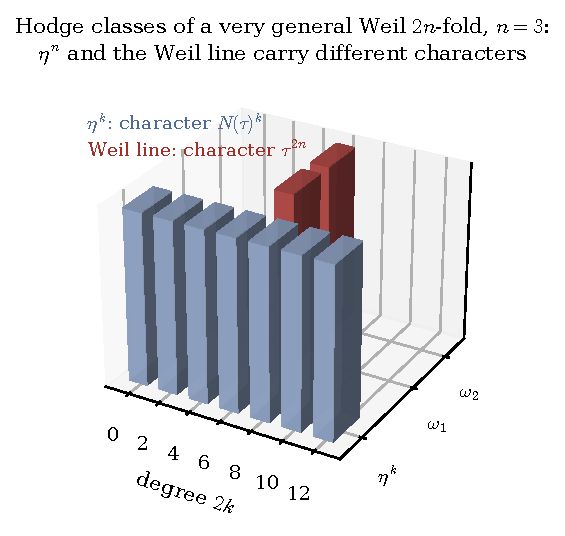
\includegraphics[width=0.92\textwidth]{figures/fig_eigen}
\caption{The Hodge classes of a very general abelian sixfold of Weil type and the characters of $K^{\times}$ on them: $\eta^{k}$ carries $N(\tau)^{k}$, the Weil plane carries $\tau^{2n}$. An eigenclass for $N^{n}$ in degree $2n$ is a multiple of $\eta^{n}$.}
\label{fig:eigen}
\end{figure*}

\paragraph{The eigencharacter (Lemmas 1, 2, Proposition 2, Theorem 4).} Equation~(1) of the preprint gives $\tau^{*}\eta=N(\tau)\eta$ for $\tau\in K^{\times}$, so $\eta^{n}$ has character $N(\tau)^{n}$, while Proposition~2 asserts character $1$. The group $K^{\times}$ acts on $W(A)=\bigwedge^{2n}_{K}H^{1}(A)$ by $\tau\mapsto\tau^{2n}$, which differs from $N(\tau)^{n}=(\tau\bar\tau)^{n}$ unless $(\tau/\bar\tau)^{n}=1$; so the Weil classes are not in the $N^{n}$-eigenspace, and an $N^{n}$-eigenclass of degree $2n$ is a multiple of $\eta^{n}$ (Fig.~\ref{fig:eigen}). The scaling of the secant sheaf by $d^{n}$ under an isogeny of degree $d$ (Lemma~1) is asserted without proof.

\paragraph{Step 4 of Theorem 4.} The points of a Shimura variety with smaller Mumford--Tate group are the points of proper special subvarieties, most of which are not of CM type; and Pohlmann's theorem \cite{Poh68} covers the CM types whose Hodge ring is generated by divisors, not all CM abelian varieties.

\paragraph{The reduction to Weil classes (Theorem 3, Section 5).} Moonen and Zarhin describe every Hodge class as a polynomial in divisor classes and Weil classes of isogeny factors in dimension at most five \cite{MZ99}, and the description is not known beyond; simple CM abelian varieties can carry Weil classes \cite{Weil77,Shi79b}; and not every factor of type IV is of Weil type.

\paragraph{Theorem 12.} The Kuga--Satake construction exists for Hodge structures of K3 type, with $h^{2,0}=1$ \cite{KS67,Del72}; Theorem~12 applies it to arbitrary primitive classes. Its algebraicity, credited there to Deligne, is open: Deligne proved that the correspondence is absolutely Hodge \cite{Del82}, and its algebraicity is known only in special families \cite{vG00,Var23}. Since the case split of Section~1.4 rests on this step for the classes of coniveau zero, it is incomplete.

None of these points is repaired here. The present paper does not use secant cycles, the eigencharacter argument or the Kuga--Satake construction outside K3 type, and it claims no case of the conjecture that is not proved in Sections~\ref{sec:reduction} to \ref{sec:f2}.

\begin{table*}[hbt!]
\centering
\caption{Every statement of the paper with its status. ``Proved'' means proved in the text from the cited results; ``open'' means not proved here or elsewhere to our knowledge.}
\label{tab:status}
\begin{ruledtabular}
\begin{tabular}{llll}
statement & where & status & what it needs \\
\colrule
$\HC\Leftrightarrow\Fii{}\wedge\Fiii{}$ & Thm.~\ref{thm:intro-reduction} & proved & -- \\
\Fii{} $\Leftrightarrow$ $\AB$ & Thm.~\ref{thm:f2isab} & proved & -- \\
six minimal sufficient sets & Prop.~\ref{prop:minimal} & proved, checked in Lean & -- \\
dichotomy of the algebraic locus & Lem.~\ref{lem:dichotomy} & proved & -- \\
\Fii{} as propagation from CM points & Thm.~\ref{thm:propagation} & proved & -- \\
Weil loci dense with CM base point & Prop.~\ref{prop:weil-dense} & proved in \cite{BMB26} & -- \\
chains make $e$ with $e^{2}\in\QQ$ algebraic & Thm.~\ref{thm:chain} & proved & a chain of the right multiplier \\
$\sqrt6$ algebraic on two-dimensional families & Thm.~\ref{thm:sqrt6} & proved & -- \\
$\sqrt5$, $\sqrt7$ algebraic on one-dimensional families & Thm.~\ref{thm:fricke} & proved & -- \\
similarities act by multipliers $d_{1}d_{2}$ & Prop.~\ref{prop:structure} & proved & -- \\
finite-group correspondences give abelian $E$ & Prop.~\ref{prop:hecke} & proved & -- \\
$\HC$ for $X\times X$, $X$ in the dihedral families & Cor.~\ref{cor:dihedral} & proved & -- \\
\Fiii{} for $S_{\lambda}$, $F=\QQ(\zeta_{7})^{+}$ or $\QQ(\zeta_{9})^{+}$, $D=D_{\infty}$ & Thm.~\ref{thm:zeta9} & proved & -- \\
where the dihedral mechanism stops & Prop.~\ref{prop:cubicstop} & proved & -- \\
\Fiii{} for $S_{\lambda}$, other cubic $F$ or other $D$ & Sect.~\ref{ssec:f3stop} & open & a non-similarity correspondence \\
\Fiii{} in general & -- & open & -- \\
product object of polarised shape & Thm.~\ref{thm:product} & proved & -- \\
direct sums never semiregular & Prop.~\ref{prop:directsum} & proved & -- \\
annihilator of the secant pieces is the product locus & Thm.~\ref{thm:annihilator} & proved & -- \\
secant and line-bundle pieces orthogonal & Prop.~\ref{prop:noorth} & false for every realisation & -- \\
(P2$'$) at a product point & Sect.~\ref{ssec:f2stop1} & open & $\Ext^{*}$ of secant sheaves \\
the Ext groups at the CM point $E_{0}^{6}$ & Lem.~\ref{lem:cmext} & proved & -- \\
no two-step cancellation of diagonal classes & Prop.~\ref{prop:twostep} & proved & -- \\
three line bundles at $E_{0}^{6}$ & Prop.~\ref{prop:separated} & proved, fail & -- \\
(P2$'$) at $E_{0}^{6}$, other configurations & Sect.~\ref{ssec:f2stop1} & open & the chain products \\
sixfold link $\Rightarrow$ exceptional classes & Thm.~\ref{thm:link} & proved & -- \\
algebraicity of the link $\xi$ & Sect.~\ref{ssec:f2stop2} & open & a cycle on $X\times X\times Z_{K}$ \\
dominant maps, blow-ups, derived equivalences preserve the defect & Prop.~\ref{prop:surgery} & proved & -- \\
exceptional classes of $X\times X$ & -- & open & -- \\
\Fii{} in general & -- & open & -- \\
the Hodge conjecture & -- & open & \Fii{} and \Fiii{} \\
\end{tabular}
\end{ruledtabular}
\end{table*}
